\section{Results}\label{sec:results}

In this paper, we designed a new interpretability technique which can be used to extract knowledge graphs from state clouds of contextual embeddings. We have noticed that NSC is able to successfully recover commonsense relations of abstraction from raw text data (e.g. "apple" IS\_A "fruit", "orange juice" IS\_A "juice", see Fig. \ref{fig:nsc_output_graph}). Additionally, we have found that for a limited number of concepts to relate, the graph search is robust with respect to the starting state. Moreover, the legibility terms included in the linear combination which comprise the search objective (e.g. arc count) successfully nudge the search towards relatively sparse outputs.

\begin{figure}[h]
    \centering
    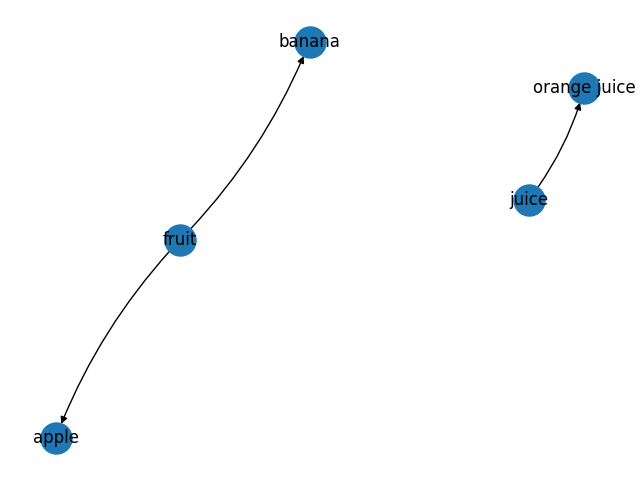
\includegraphics[width=0.45\textwidth]{img/distinct graphs.png}
    \caption{NSC output graph when applied to BERT using several symbols.}\label{fig:nsc_output_graph}
\end{figure}

Additionally, the graph search history profile exhibits proper foraging behavior, with fast increases in solution quality in the beginning, followed by a more conservative strategy which ends in marginal improvements towards the move to heavy exploitation (see Fig. \ref{fig:nsc_score_history}).

\begin{figure}[h]
    \centering
    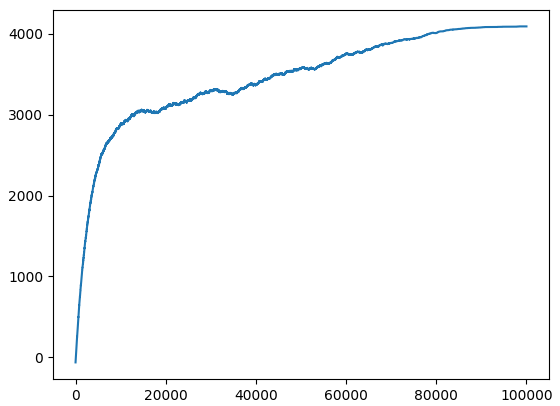
\includegraphics[width=0.45\textwidth]{img/score1.png}
    \caption{Candidate score by epoch during the graph optimization process.}\label{fig:nsc_score_history}
\end{figure}

\textbf{A graph optimization run with the same hyperparameter configuration and different targeted concepts resulted in a similar graph output (see Fig. \ref{fig:valuable}). Interestingly enough, while every single arc present in the output graph depicts a valid relation of abstraction (e.g. "food" $>$ "vegetable", "vegetable" $>$ "onion", etc.), the graph still has several shortcomings. The implicit structure of the concepts analysed would reflect the three vegetables mentioned (i.e. "carrot", "potato", and "onion") as children of the "vegetable" node. However, two of them (i.e. "carrot" and "potato") have been linked directly to the more abstract "food".}

\begin{figure}[h]
    \centering
    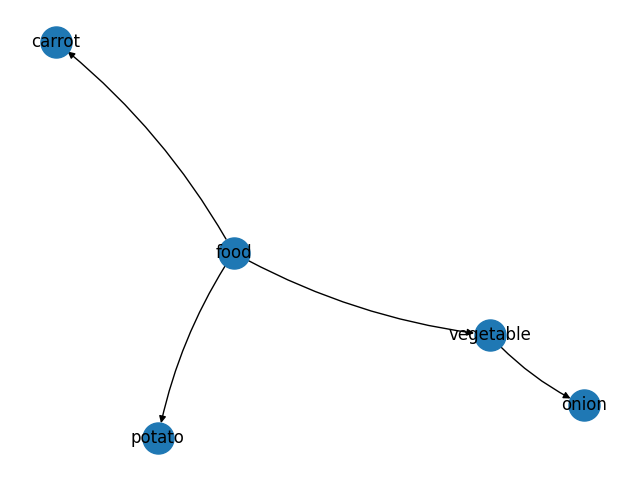
\includegraphics[width=0.45\textwidth]{img/valuable contrasts.png}
    \caption{NSC output graph when applied to BERT using several symbols.}\label{fig:valuable}
\end{figure}

\textbf{This likely reflects a limitation of the objective function we employed. Namely, the four terms of the linear combination (i.e. expressed abstraction, arc density, children error, and parent error) have collectively proven insufficient for capturing and incentivizing this implicit structure. It appears more valuable for the graph optimization algorithm in terms of the objective function to populate the graph with arcs which denote particularly \textit{abrupt} relations of abstraction. In this last graph output (see Fig. \ref{fig:valuable}), this is reflected in the favoring of the ("food", "potato") arc over the $\{("food", "vegetable"), ("vegetable", "potato")\}$ pair of arcs. Alternatively, arc density could be penalized less in order to render this arc pair more appealing in contrast to the single more abrupt arc.}

\textbf{Besides the final graph output generated by NSC, we can also investigate the intermediate step of estimating the relation of abstraction between two concepts. If we zoom into the pairwise estimate of abstraction between "vegetable" and "carrot", we can observe a promising pattern. We consider the difference matrix $D = C_{vegetable} - C_{carrot}$, where the two $C$ matrices correspond to the matrices of the conceptors obtained for the two concepts based on their associated exemplars. If we derive and plot the eigenvalues $\{\lambda_{i}(D)|i \in \{1, 2, ... d_{BERT}\}\}$ of the previous difference matrix, we notice that their mean (denoted by the horizontal red line in the Fig. \ref{fig:spectrum}) is positive. However, we also notice that there is an important number of negative eigenvalues as well, hinting at the value of improving the noise robustness of NSC.}

\begin{figure}[h]
    \centering
    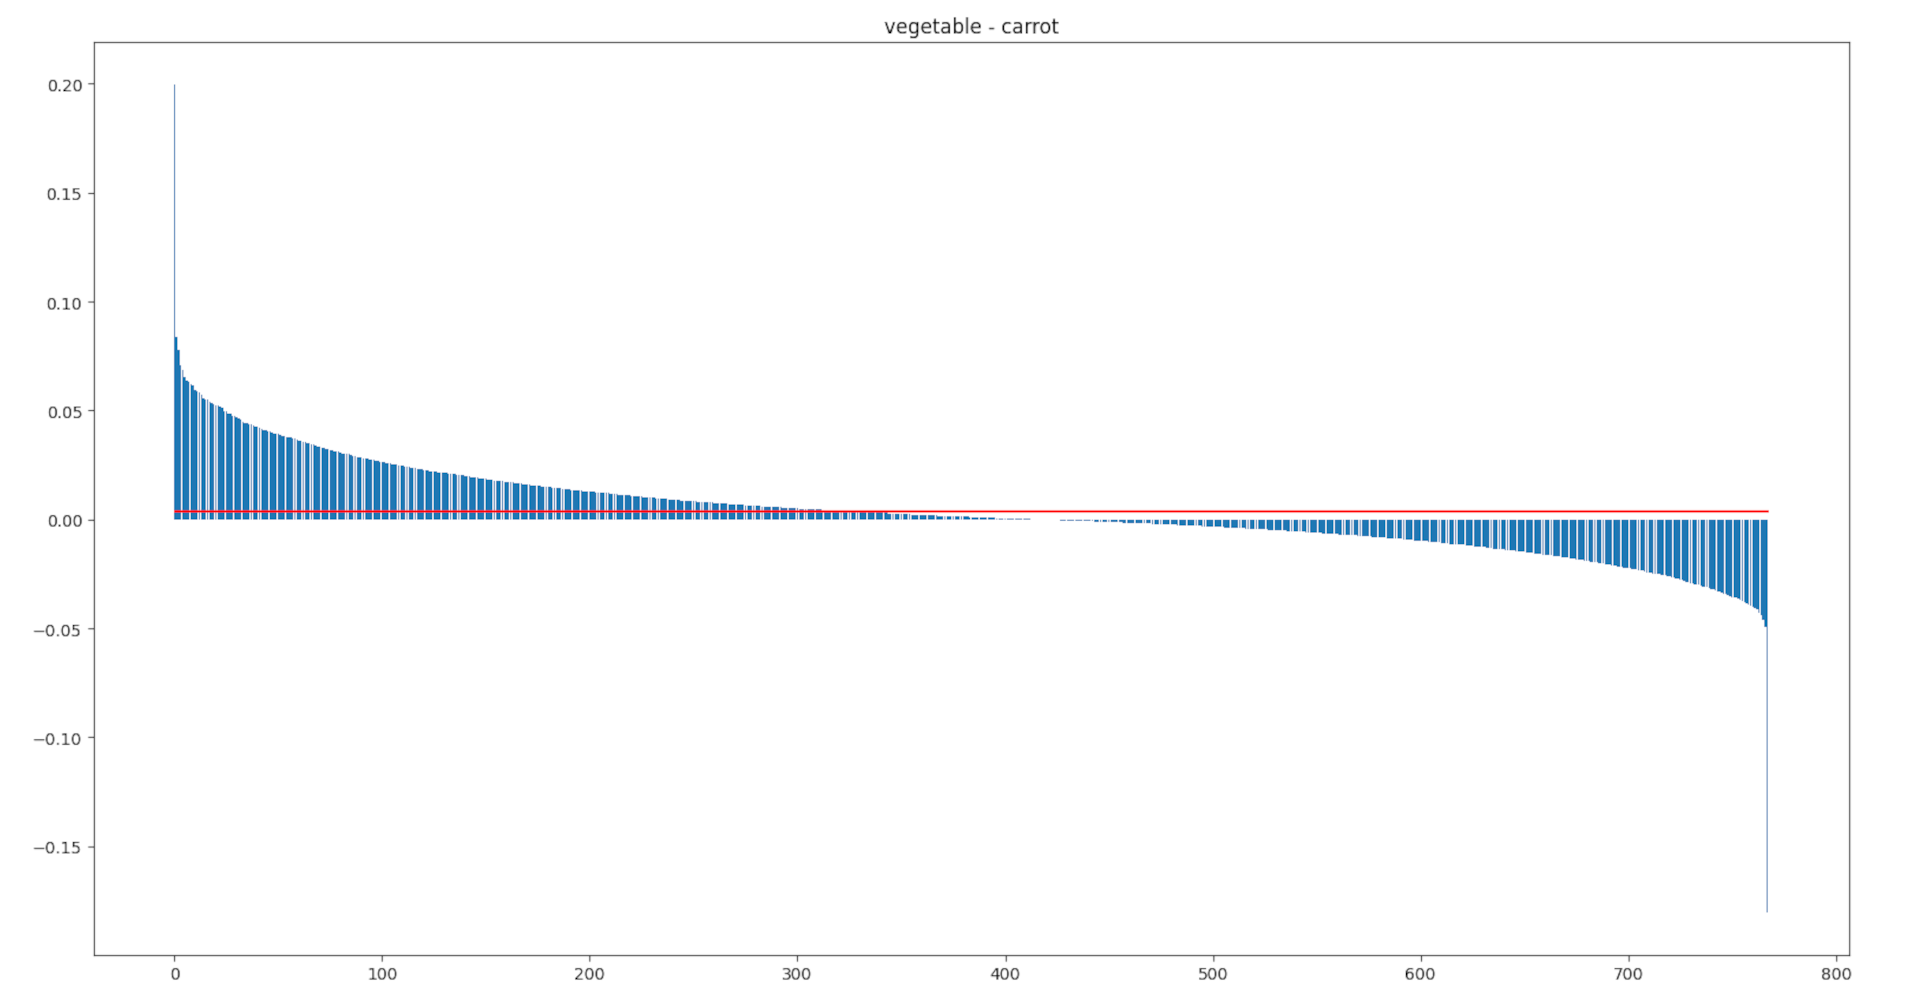
\includegraphics[width=0.45\textwidth]{img/spectrum.png}
    \caption{NSC output graph when applied to BERT using several symbols.}\label{fig:spectrum}
\end{figure}

Additionally, we took note of the fact that the graph optimization process employed to output the final knowledge graph is highly sensitive to the precise choice of the objective function. Striking a balance between the legibility terms and the expressed abstraction is difficult to achieve manually. Often, one component of the linear combination tends to dominate the others. For instance, undervaluing the impact of the children error (i.e. the term which nudges the optimization process towards graphs whose nodes have a specific number of children) fails to penalize graphs which contain nodes with either numerous children or none at all (see Fig. \ref{fig:children}).

\begin{figure}[h]
    \centering
    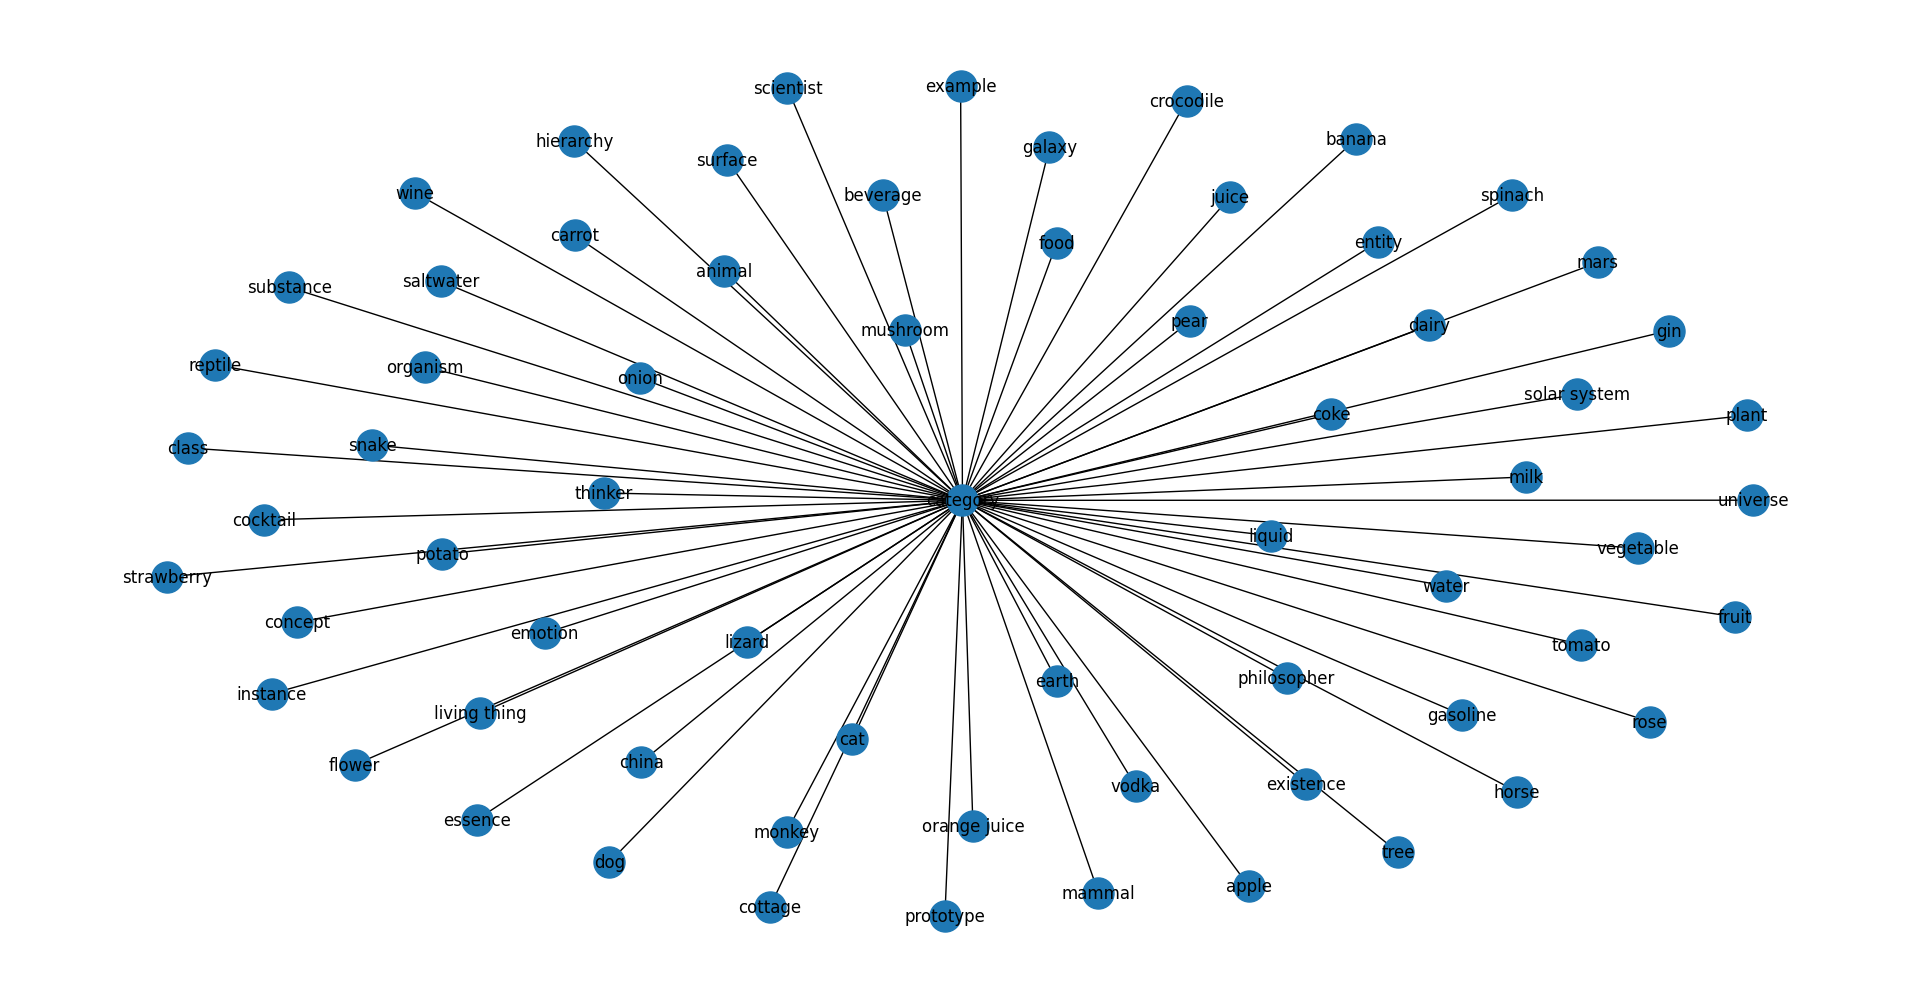
\includegraphics[width=0.45\textwidth]{img/too_much_pruning.png}
    \caption{NSC output graph after undervaluing children count per node constraints.}\label{fig:children}
\end{figure}

\textbf{A similar failure mode manifested itself when undervaluing the impact of arc density on graph optimization (i.e. the term which nudges the optimization process towards graphs which are sparse, in that they contain a relatively low number of arcs connecting nodes). In this other case, the optimization process favored graphs which contain many arcs (Fig. \ref{fig:pruning}). We speculate that this happened because considering candidate graphs which contain many arcs translates to an increase in expressed abstraction. In other words, simply including arcs which connect concepts which seemingly have a positive relation of abstraction (i.e. the arc's origin node is the slightest more abstract than the arc's target node) yield increases in terms of the objective function. Without a comparable arc density penalty, the optimization process approaches graphs overpopulated by arcs.}

\begin{figure}[h]
\centering
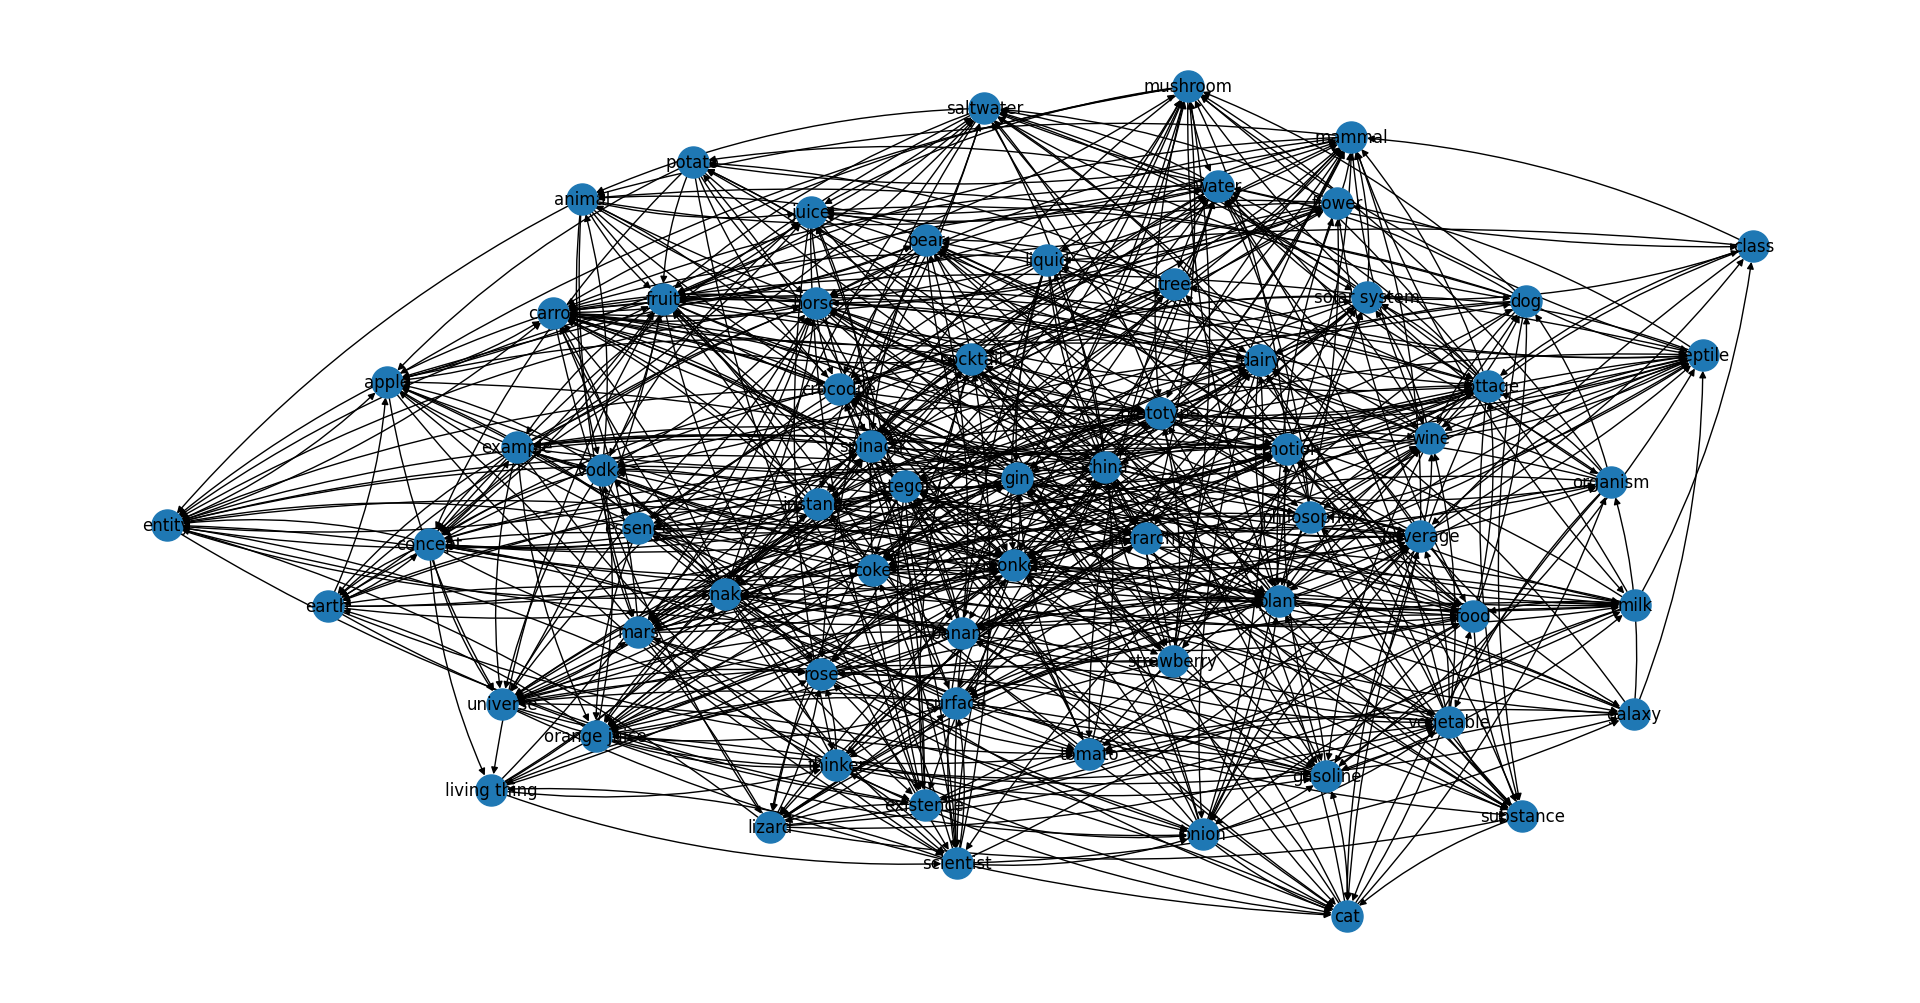
\includegraphics[width=0.45\textwidth]{img/short_run.png}
\caption{NSC output graph after undervaluing arc pruning.}\label{fig:pruning}
\end{figure}

\textbf{This sensitive balance between the competing terms which make up the objective function echoes a broader concern which permeates XAI. There is a constant trade-off between functional-groundedness and human-groundedness which resembles the adequacy-fluency trade-off frequent in machine translation. In our case, the expressed abstraction term incentivizes functional-groundedness, the adequate communication of high-dimensional relations among concepts. In contrast, the three legibility terms employed in the objective function incentivize human-groundedness, the communication of DL model representations in a manner which is cognitively ergonomic for humans. 
}

\textbf{In our experiments, we find that striking this balance is especially difficult when trying to distill larger knowledge graphs containing more concepts from high-dimensional embeddings, bringing the scalability of NSC into question. That said, normalizing the objective's components relative to the total number of concepts being analyzed (i.e. all legibility terms assume values in $[0, 1]$ before weighting, regardless of node count) did improve scalability.}
